\section{Theorie}

\subsection{Das grundsätzliche Prinzip des Photoeffekts}

    Licht hat zwei unterschiedliche Erscheinungsformen:
    Zum einen das Wellenbild,
    welches Phänomene wie Beugung und Interferenz erklärt,
    zum anderen das korpuskulare Modell,
    also das Teilchenmodell,
    mit dem sich der Compton-Effekt, die Paarbildung und der Photoeffekt erklären lassen.\\
    Je nach dem Versuch ist entweder das Wellen- oder das Teilchenbild relevant.
    Für den Photoeffekt ist das Teilchenbild des Lichts entscheidend.\\
    Der generelle Aufbau zur Messung des Photoeffektes ist in Abbildung \ref{fig:genAufbau} gezeigt.

    \begin{figure}
        \centering
        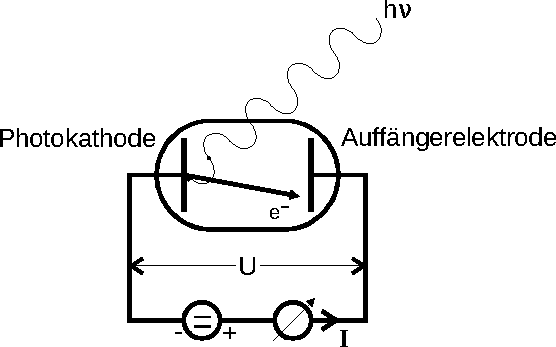
\includegraphics[width=\textwidth]{content/img/Abb_1.pdf}
        \caption{Grundlegender Aufbau zur Messung des Photoeffektes.}
        \label{fig:genAufbau}
    \end{figure}

    Im Vakuum wird eine negativ geladene Photokathode mit monochromatischem Licht aus einer Quelle bestrahlt.
    Das Licht besteht nach dem Teilchenmodell aus Photonen,
    oder auch Lichtquanten genannt,
    die eine diskrete Energie $E_\text{Ph}$ besitzen.
    Wenn die Photonen auf die Photokathode treffen,
    können sie,
    sofern ihre Energie groß genug ist,
    Elektronen aus dem Material der Photokathode herauslösen.
    Wenn $E_\text{Ph}$ größer als die Austrittsarbeit $A_\text{K}$ der Elektronen ist,
    wird die zusätzlich übertragene Energie in kinetische Energie $E_\text{Kin}$ der Elektronen umgewandelt
    \begin{equation}
        E_\text{Ph} = h \nu = A_\text{K} + E_\text{Kin} . \label{eqn:Photonenenergie}
    \end{equation}
    Der Zusammenhang zwischen der Frequenz $\nu$ und der Wellenlänge $\lambda$ ist durch
    \begin{equation*}
        \nu = \frac{c}{\lambda}
    \end{equation*}
    gegeben,
    mit der Lichtgeschwindigkeit $c = \SI{3e8}{\meter\per\second}$.
    Die Elektronen fliegen zu einer positiv geladenen Anode,
    an der ein Photostrom der herausgelösten Elektronen zu messen ist.
    Wenn $E_\text{Ph}$ kleiner als $A_\text{K}$ ist,
    können die Elektronen nicht herausgelöst werden,
    es existiert also eine Grenzfrequenz,
    ab der der Photoeffekt erst möglich ist.
    Zusätzlich gilt,
    dass die Lichtintensität proportional zur Anzahl der Photonen pro Zeit- und Raumwinkel ist.
    Außerdem kann pro Photon nur ein Elektron herausgelöst werden,
    woraus folgt,
    dass die Anzahl der pro Zeit herausgelösten Elektronen proportional zur Lichtintensität ist.
    Aus der Gleichung \eqref{eqn:Photonenenergie} folgt,
    dass die kinetische Energie der Elektronen abhängig von der Frequenz $\nu$ des Lichts ist,
    mit dem die Photokathode bestrahlt wird.

\subsection{Experimentelle Messung des Photoeffektes mit der Gegenfeldmethode} \label{sec:zweizwei}

    Zur Untersuchung des Photoeffektes wird die sogenannte Gegenfeldmethode verwendet.
    Dazu wird ein variables Potential $U$ zwischen Photokathode und Anode (siehe Abbildung \ref{fig:genAufbau}) angelegt,
    welche dazu führt,
    dass die herausgelösten Elektronen durch ein gegengerichtetes elektrisches Feld abgebremst werden.
    Dies sorgt dafür,
    dass der gemessene Photostrom kleiner wird,
    da nur noch Elektronen,
    deren Energie groß genug ist das Feld zu überwinden,
    auf der Anode auftreffen.
    Der Photostrom verschwindet,
    wenn
    \begin{equation}
        e_0 U_\text{g} = \frac{1}{2} m_0 v_\text{max} ^2
    \end{equation}
    gilt,
    also auch die Elektronen mit der größten Geschwindigkeit $v_\text{max}$ bei einer Grenz-Gegenspannung $U_\text{g}$
    die Kathode nicht mehr erreichen.
    Dabei ist hier $e_0$ die Elementarladung der Elektronen und $m_0$ ihre Ruhemasse.
    Die Energie der schnellsten Elektronen kann durch
    \begin{equation}
        h \nu = A_\text{K} + e_0 U_\text{g}
    \end{equation}
    berechnet werden.\\
    Der Photostrom fällt bei steigender Gegenspannung $U$ allerdings nicht sofort ab, wie in Abbildung \ref{fig:GegSpannungStrom} gezeigt,
    was daran liegt,
    dass die Elektronen im Material verschiedene Energieniveaus besitzen und daher verschiedenenergetisch sind,
    wenn sie aus der Photokathode herausgelöst werden.

    \begin{figure}
        \centering
        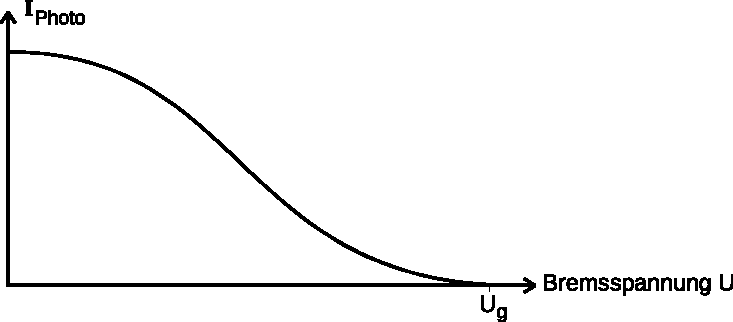
\includegraphics[width=\textwidth]{content/img/Abb_5.pdf}
        \caption{Verlauf des Photostroms bei steigender Gegenspannung.}
        \label{fig:GegSpannungStrom}
    \end{figure}
    %\clearpage

    Die Energieverteilung der Elektronen im Material kann mit der Fermi-Dirac-Statistik erläutert werden.
    Sie besagt, dass sich die Energie der Elektronen auf einem Intervall von 0 bis zu einer Fermi-Energie $\zeta$ beschreiben lässt.
    Die obere Grenze $\zeta$ ist materialabhängig.
    Die herausgelösten Elektronen haben teilweise also eine Energie, die größer als $h \nu - A_\text{K}$ ist.\\
    Für den Photostrom ergibt sich folgender Zusammenhang
    \begin{equation}
        I_\text{Ph} \propto U^2 .
    \end{equation}
    In einem Diagramm von $\sqrt{I_\text{Ph}}$ gegen $U$ bildet $U_\text{g}$ die Nullstelle (siehe Abbildung \ref{fig:GegSpannungStrom}).\\
    \\
    Zusätzlich muss in manchen Fällen eine Beschleunigungsspannung $U_\text{b}$ angelegt werden,
    damit Photostrom ensteht und
    \begin{equation}
        h \nu + e_0 U_\text{b} \geq A_\text{A}
    \end{equation}
    ist.
    Die Energie der Elektronen, welche sich aus $E_\text{Ph} =  h \nu$ und der elektrischen Energie $e_0 U_\text{b}$ zusammensetzt,
    muss größer sein als die Austrittsarbeit $A_\text{A}$ der Anode sein,
    damit die Elektronen auf die Anode treffen.
